\section{The Concept and Properties of Digital Identity}

The identity concept can be seen from different perspectives and is applicable in different domains, depending on the objective for which digital identity is used. In general, personal identity in philosophy refers to the answer to the question, ‘Who am I?’ It consists roughly of those properties that make the individual unique and different from others[7]. Precisely, identity refers to a set of qualities and characteristics that make an entity definable, distinguishable, and recognizable compared to other entities[8]. However, in the digital world, “identity” is a set of digital records that represents a user. These records are saved and managed in a standard format by entities that provide the identity information or assurances needed to complete transactions. Digital identity also accepts and integrates new records to create a rich view of the user[9]. The following are five properties that should be applied to contribute to a more detailed and provisioning solution of a digital identity system.

\subsection{Entities}

According to its definition, an entity is an object that exists or has its own independent existence. Entity conduct as representation from a unit that bears the legal rights for the system, e.g., individuals, businesses, and affiliates. Those entities can be specifically categorized into three types[10]. They have their own private and public keys and can be run by parties that have certain user credentials, such as banks, universities, or other entities that are trusted by the user. The last type consists of Relying parties, which represent a party with which a user intends to interact, essentially, an online service provider; however, in a peer-to-peer system, relying parties can be other users.

\begin{figure}[H]
    \centering
    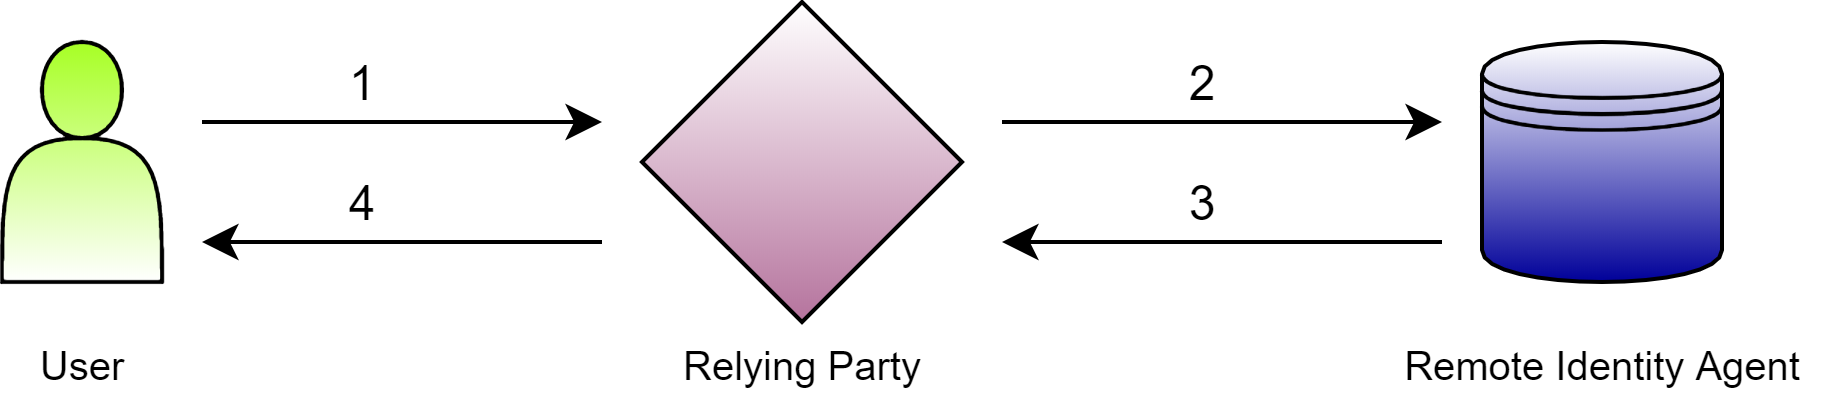
\includegraphics[scale=1]{3.png}
    \caption{Entities}
    \label{fig:threshold}
  \end{figure}

 \subsection{Attribute Type}

 The attribute type is used to identify the entity. There are three major types[11].

 \subsubsection{Who you are}
 In the real world, it is easy to identify a single entity  It can include knowledge or data that is only known by that entity, unique physical characteristics of that entity, or items that the entity possesses.

 \subsubsection{Context}
 Different constraints on digital identity may be implemented depending on the context. For instance, transferring sensitive information relating to birth certificates over the phone or the internet may be prohibited. level of trust is play a major role here, so the context is used to identify the quantity and type of information needed for providing the trust. For example, in an email context, the amount of identifying information necessarily is usually only two things: a username and a password. 

 \subsubsection{Profile}
 After user is verified the profile data is needed for services. User profiles can include what entities can do, what they have subscribed to, what groups they are members of, their selected services, etc. A user’s profile can change during the course of an interaction with the service provider.

\subsection{Lifecycle}
There are three fundamental steps to creating digital identity[12]: registration, including enrollment and validation; issuance of documents or credentials; and authentication for service delivery or transactions.

\begin{figure}[H]
    \centering
    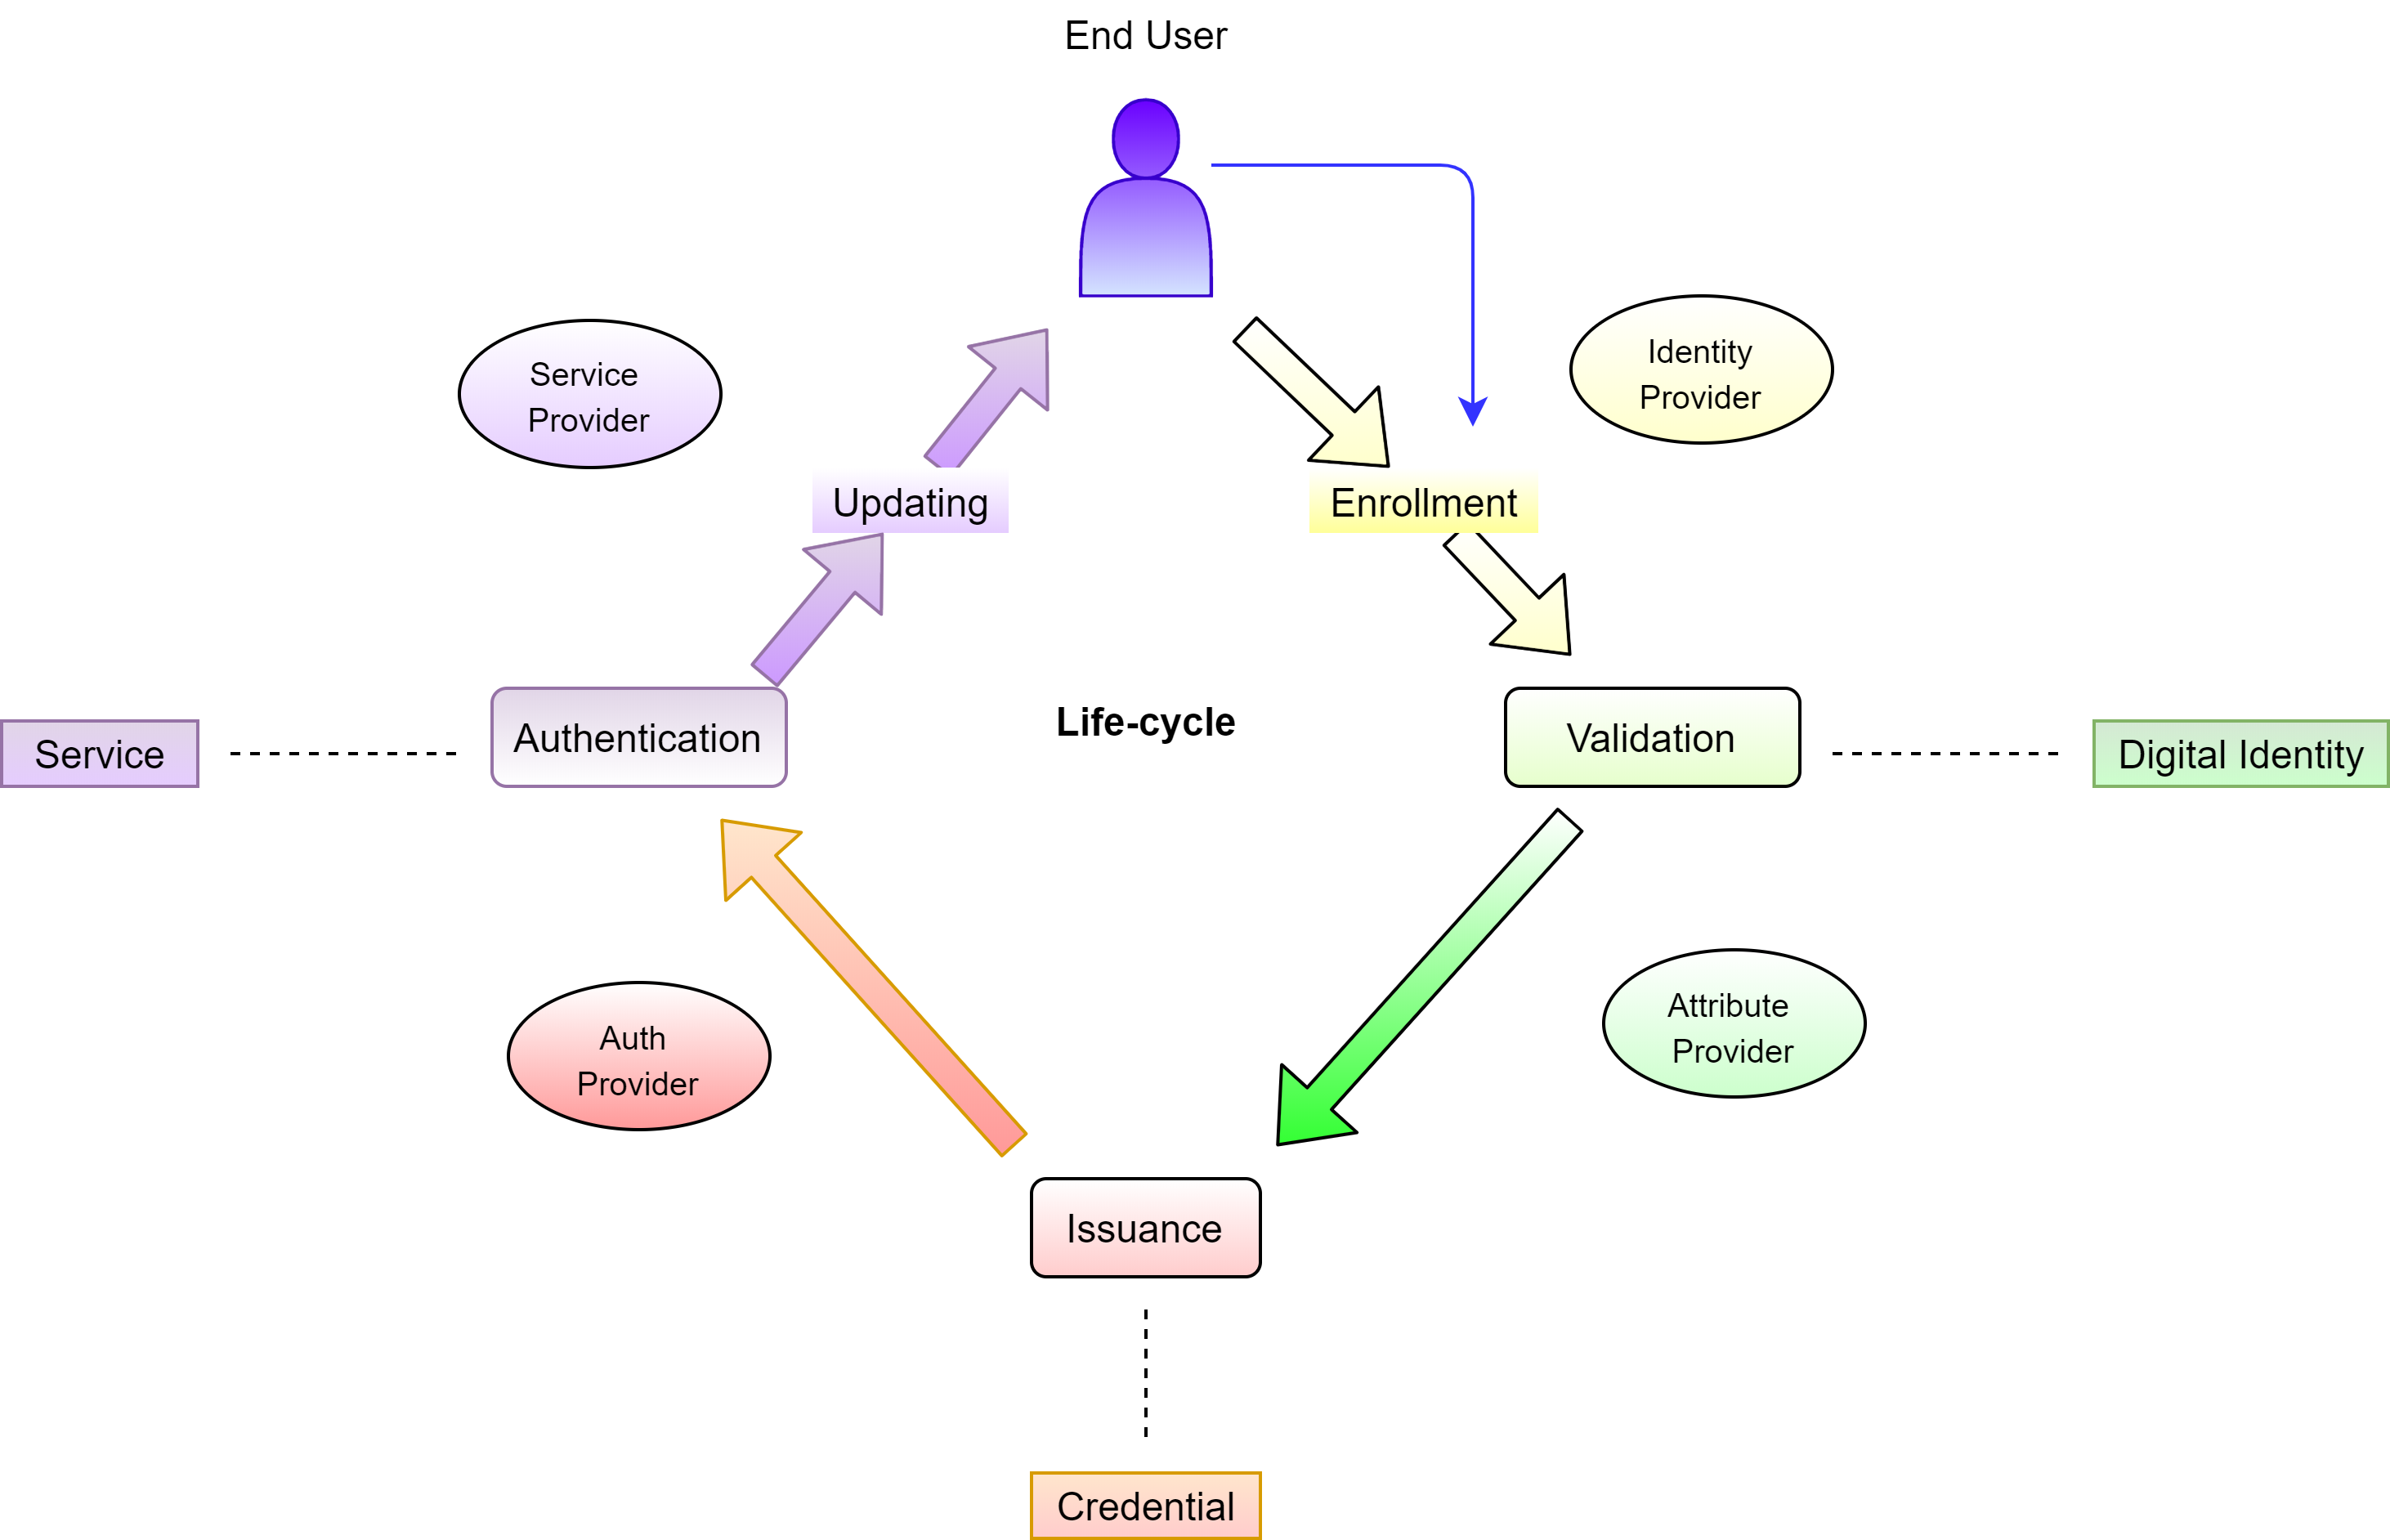
\includegraphics[scale=0.8]{4.png}
    \caption{Digital Identity Lifecycle}
    \label{fig:threshold}
  \end{figure}

  \subsubsection{Enrollment}
  There are two main categories, which are enrollment and validation. Enrollment registration steps: capturing and recording key identity attributes of a person who claims a certain identity. This may include biographical data (e.g., name, date of birth, gender, address, email), biometrics (e.g., fingerprints, iris scan), and the other attributes. 
  
  \subsubsection{Issuance}
  Before it can be used by a person, a registered identity goes through an issuance or credentialing process. For an identity to be considered digital, the credentials or certificates (e.g., birth certificate, passport) issued must be electronic, in the sense that they store and communicate data electronically. Types of electronic credentials including smartcards, 2D barcode cards, mobile identity, and identity in the cloud.

  \subsection{Policies}
  The level of access is conditioned not only by the identity but is also likely constrained by a number of further security considerations, such as the company policy.
  
  \subsection{Technology}
  \subsubsection{Authentication Techniques}
  The authentication processors were varying from different factors. the list of major methods are listed below

  \begin{itemize}
      \item Password or personal identification number (PIN)
  \end{itemize}

  This advanced method involves hashing and the techniques and data are then exchanged with the server and stored [10]. The PIN technique basically has the same mechanism as a password, but it consists of a numeric term only (usually with four to six digits). still, in the world, the pin-based process is following in banks and other business industries. 

  \begin{itemize}
    \item Token
\end{itemize}
  
This works using the two-factor authentication (2FA) principle. Instead of using a username and password, a level is added on to obtain a time-limited token (typically a cryptographic key or password) that is used for further transactions during the session. The physical device for tokens mostly does not require an internet connection because it communicates using mobile telecommunication service operator services such as voice calls, SMS, or USSD. 

\begin{itemize}
    \item Public key cryptography
\end{itemize}

This method utilizes cryptographic mechanisms that, as their underlying theory, engage an asymmetric key pair: a public key and a private key [13]. using the key pair, data encryption and decryption can be done as well as the signing the data can be done using these key pairs.

\begin{figure}[H]
    \centering
    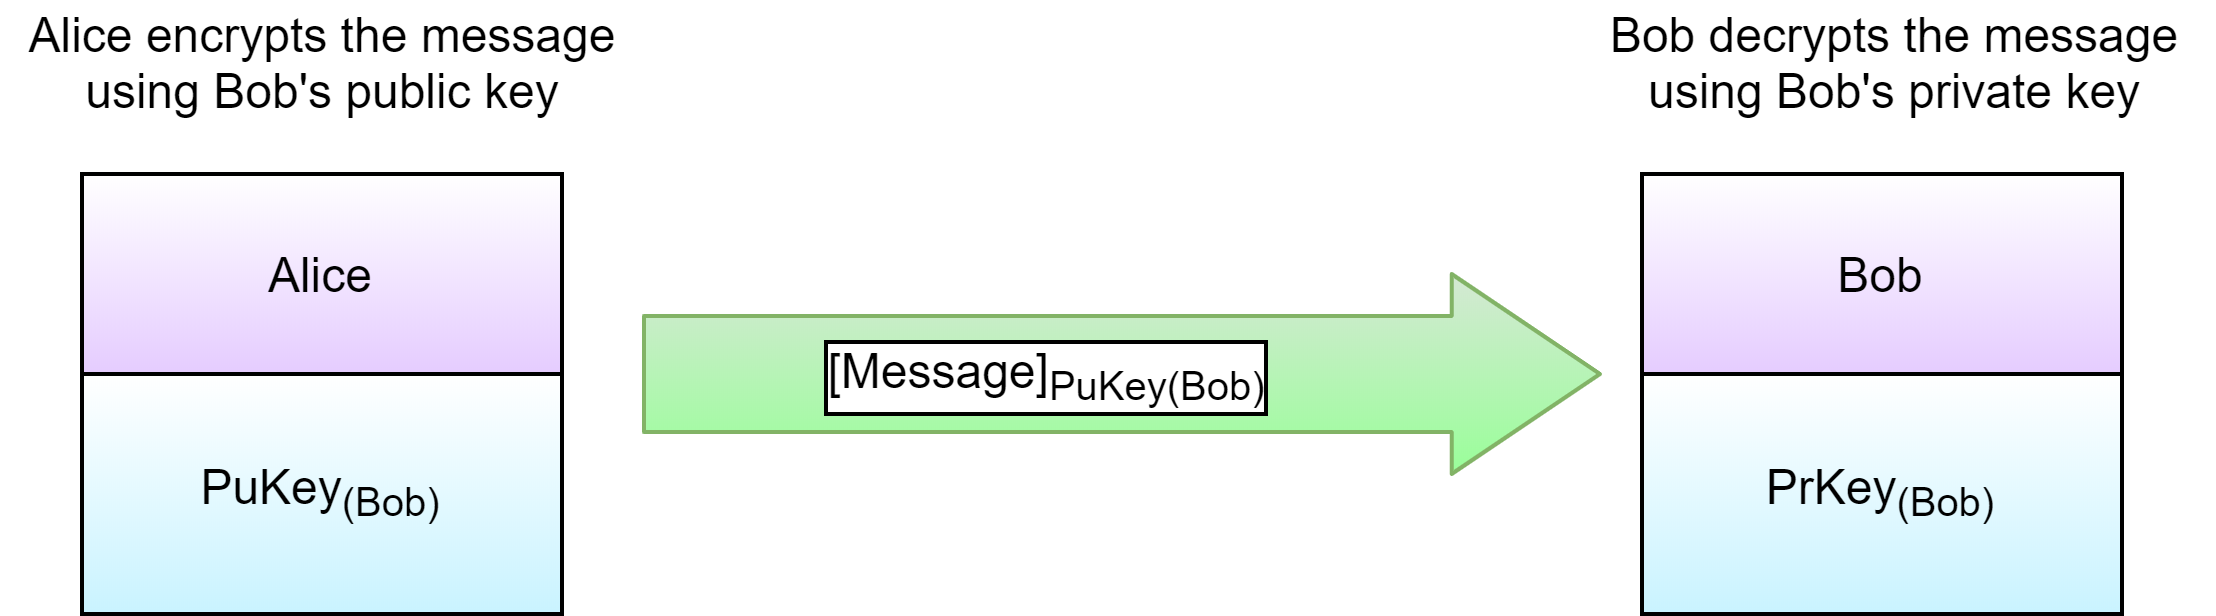
\includegraphics[scale=0.8]{5.png}
    \caption{Keypair cryptography}
    \label{fig:threshold}
  \end{figure}

  \begin{itemize}
    \item Biometric
\end{itemize}

Biometric authentication requires a completely different style of the authentication process. This approach is based on a person’s biological uniqueness and it can be used for the biometric identification of a person [14], using, for example, fingerprint or iris recognition.most of the pattern matching techniques used for this. Biometrics also depends on the devices that are collect data.

\begin{itemize}
    \item Smart Card
\end{itemize}

When used for logical access, smart card technology typically comes in two forms: a credit-card-sized plastic card or a USB device, each with an embedded computer chip [15]. the major application of a smart card is storing a password.

\subsubsection{Security Protocols}

security protocols highly valued because verification and authentications are depended on that. The widespread authentication protocols used to address security issues within open networks are Secure Sockets Layer (SSL), IP Sec, Secure Shell (SSH), and Kerberos [16]. 

\subsubsection{Storage}

There are two new technologies that may offer improved methods in database storage [9]. The first is distributed ledger technology or blockchain combined with encryption and cloud storage, and this allows information to be held and transferred point-to-point in a dispersed, immutable network. The second consists of federated identity standards, such as SAML 2.0, which create interoperability between identity management networks and external applications, allowing federated identity systems to scale to accommodate large numbers of identity providers and relying parties.

single-sign-on (SSO) authentication. plays a major role in the authentication context in this era. This system allows users to sign on only once and have their identities automatically verified by each application or service they want to access afterward[17]. This system serves different purposes[18]. It communicates between applications and the network, it enables communication to applications that are connected by the internet using web resources, and it integrates different domains with different sets of credentials located all over the world. The aim of using SSO is to improve the communication and security of user authentication and access permission verification and also to decrease management costs [19]. Popular examples of SSO systems are found at Google, Microsoft, Facebook, and Yahoo; they provide SSO to their users when accessing emails, groups, documents, and other facilities embedded in their SSO system



  

  